\section{A Multi-Channel Sparse Blind Deconvolution approach to STM}

In this chapter, we will introduce our approach to address \ac{MC-SBD} problem. We will first analyze the bi-linear nature of \ac{MC-SBD}, overview the possible methods that address it. We then briefly introduce Riemannian Trust Region method(RTRM), a direct non-convex optimization algorithm that addresses \ac{SBD} problem. Finally, we present our algorithm which extends \ac{RTRM} to multiple channel cases. 

\ac{MC-SBD}, also known as the joint sparse blind deconvolution/demixing problem is a bi-linear problem, that is, the observed signal is modeled as a convolution (or equivalent linear operation) between pairs of two unknowns—and this operation is linear in each variable when the other is fixed, but not jointly linear. Bi-linear problems can be solved by either a lifted method or a direct method. A lifted method can formulate the initial bi-linear mapping of two unknowns to a linear mapping of a single unknown, by defining a one-to-one mapping from two unknowns to the targeted unknown. For example, given observation $y = \mathbb{A}(x,h)$, where $x \in \mathbb{R}^n$ and $h \in \mathbb{R}^m$ are two inputs we tries to recover. We can define an outer product $X = xh^T\in \mathbb{R}^{n\times m}$, and rewrite observation $y = \mathbb{A'}(X)$. In the case of convolution, $\mathbb{A'}$ is the Lifted circular convolution operator. A lifted problem is easier to solve analytically, and since we are dealing with only one subspace defined by $X$, by assigning constrains on $(x,h)$,  $X$ usually present some internal structures, and we are left with a fully convex problem; thus, the convergence to global minimum can usually be proven, this is also known as the recovery guarantee. For example, Flinth et al. shown that, given both inputs sparse, they can achieve high probability recovery by lifting the \ac{MC-SBD} problem and applying a hierarchical sparsity framework[tocite]. 

However, in real cases, it is rare to find both inputs sparse. Moreover, the lifting method is normally computationally inefficient, as the dimension of output space is the product of two separate inputs, it expands quickly with higher input dimensions, making it unfavorable for larger size problems like the QPI-STM recovery. On the contrary, a direct method updates one input while assuming the other one fixed, the optimization space of the problem thus grows linearly with the input dimension. The trade off is that with direct methods, recovery guarantee is hard to obtain, instead, local minimal recovery can be guaranteed with careful algorithm design. Local convergence can be combined with an initial guess that is close to the global minimum; this recipe of combining good initial guesses and an algorithm with strong guarantees of local convergence usually leads to good recovery. 

Our algorithm is a direct method that follows the above recipe, it utilizes Riemannian Trust Region Method(RTRM) to provide local convergence. Standard Trust Region Method is a second-order method that guarantees local minimum recovery, as long as the objective(ie, the cost function $\phi$) has no degenerate stationary points, that is, the Hessian $\Delta^2\phi$ has no zero eigenvalues. This ensures a sufficiently curved optimization landscape for the algorithm to make consistent progress. Moreover, compared to first-order methods based on gradient descent, Trust Region Methods has significantly faster convergences and a better overall tail convergence when the iterates are close to local minima. 

\ac{RTRM} is first raised by Absil et al. in 2007 as the extension of Trust Region Methods on a Riemannian sub-manifold, embedded in Euclidean spaces. This is advantageous since enforce our manifold to follow certain geometry, for example in our case, we enforce the kernel to live on a hypersphere $S$ defined by Equation \ref{hypersphere}, which removes the scaling symmetry we discussed. As a result, the \ac{RTRM} provides strong guarantees that a local minimum of the objective be attained over S. We now present the \ac{RTRM} algorithm used by Cheung et al. \cite{cheungDictionaryLearningFouriertransform2020} that addresses \ac{SBD} problem; we then build on it and present our \ac{MC-SBD} algorithm. 

\subsection{SBD algorithm}
Recall we have the objective function $\phi_{\lambda}$: 
\begin{equation}
	\phi_{\lambda} = \frac{1}{2}\left\lVert A_0 * X_0 - Y \right\rVert^2_F + \lambda \cdot  \left\lVert X\right\rVert_1,
\end{equation}
since \ac{RTRM} is a second-order method, we need to make make our objective function smooth, more particular, we need to smooth the sparse regularizer. This can be achieved by approximate the $l_1-norm$ by $r_{\mu}(X)$:
\begin{equation}
	r_{\mu}(X) \equiv \sum_{i,j} \mu^2(\sqrt{1+\mu^{-2}\cdot X_{i,j}}-1), 
\end{equation}
this is called a pseudo-Huber regularizer, in the limit of $\mu -> 0$, the regularizar resembles $l_1-norm$, in our case, we choose $\mu = 10^{-6}$. 

To adopt a direct method as we discussed, we will updates each input to minimize the objective function while assuming the other input fixed. We now solve: 
\begin{equation}
	\label{sbdalgorithm}
	(\hat{A}, \hat{X}) \leftarrow \min_{{A} \in {S}} \left\{ 
	\phi_{\lambda}({A}) \equiv \min_{X} \left[ 
	\phi_{\lambda}({A}, {X}) \equiv \frac{1}{2} \left\| {A} * {X} - {Y} \right\|_F^2 
	+ \lambda \cdot r_{\mu}({X}) 
	\right] 
	\right\}.
\end{equation}
This updating algorithm consists of an inner and an outer solver. The inner solver: $X \leftarrow \mathbf{XSolve}(A_{i}, \lambda)$, that is, obtaining $\hat{X}$ that minimizes $\phi_{\lambda}(A_{i},X)$ using \ac{RTRM}. The outer solver: $A_{i+1} \leftarrow \mathbf{ASolve}(A_{i}, \hat{X}, \lambda)$, obtaining $A_{i+1}$ that minimizes $\phi_{\lambda}(A_{i},X)$ using \ac{RTRM}. Since $\mathbf{XSolve}$ is an intermediate step, we can simply write the whole process as: $A_{i+1} \leftarrow \mathbf{ASolve}(A_{i}, \lambda; Y,(m_1,m_2))$, where $(m_1,m_2)$ is the predefined kernel size. 

We can then write the Complete SBD-STM procedure: 

\begin{algorithm}
	\label{SBDalgo}
	\caption{Complete SBD-STM Procedure}
	\textbf{Input:}
	\begin{itemize}
		\item Observation $Y \in \mathbb{R}^{n_1 \times n_2 \times s}$,
		\item Kernel size $(m_1, m_2)$,
		\item Initial $\lambda_0 \geq 0$, decay rate $\alpha \in [0,1)$, and final $\lambda_{\text{end}} \geq 0$.
	\end{itemize}
	
	\textbf{Phase I:}
	\begin{enumerate}
		\item Randomly initialize: $A^{(0)} \in S = \mathbb{S}^{m_1 \times m_2 \times s}$.
		\item $A_\star^{(0)} \leftarrow \texttt{ASolve}(A^{(0)}, \lambda_0)$.
	\end{enumerate}
	
	\textbf{Phase II:}
	\begin{enumerate}
		\item Lifting: Get $A^{(1)} \in S' = \mathbb{S}^{m_1' \times m_2' \times s}$ by zero-padding the edges of $A_\star^{(0)}$ with a border of width $\left\lfloor \frac{m_1}{2} \right\rfloor$.
		\item Set $\lambda_1 = \lambda_0$.
		\item Continuation: \textbf{Repeat} for $k = 1, 2, \dots$ \textbf{until} $\lambda_k \leq \lambda_{\text{end}}$,
		\begin{enumerate}
			\item[(a)] $A_\star^{(k)} \leftarrow \texttt{ASolve}(A^{(k)}, \lambda_k)$,
			\item[(b)] \textbf{Centering}:
			\begin{enumerate}
				\item[i.] Find the size $m_1 \times m_2$ submatrix of $A_\star^{(k)}$ that maximizes the Frobenius (square) norm across all $m_1 \times m_2$ submatrices.
				\item[ii.] Get $A^{(k+1)}$ by shifting $A_\star^{(k)}$ so that the chosen $m_1 \times m_2$ restriction is in the center, removing and zero-padding entries as needed.
				\item[iii.] Normalize $A^{(k+1)}$ so it lies in $S'$.
			\end{enumerate}
			\item[(c)] Set $\lambda_{k+1} = \alpha \lambda_k$.
		\end{enumerate}
	\end{enumerate}
	
	\textbf{Output:}
	\begin{itemize}
		\item Extract $\hat{A} \in S$ by extracting the restriction of the final $A^{(k+1)}$ to the center $m_1 \times m_2$ window.
		\item Find the corresponding activation map $\hat{X} \in \mathbb{R}^{n_1 \times n_2}$ by solving $\min_{X} \psi_{\lambda_k}(\hat{A}, X)$.
	\end{itemize}
\end{algorithm}

The kernel is first randomly initialized and feed into two phases sequentially. Both phases utilize the same core algorithm $\mathbf{ASolve}$ as described above; phase I aims to obtain a primary kernel $A^{(0)}_*$. Phase II serve as a refinement that increases the recovery quality by applying a stricter sparsity regularizer, as well as addresses the degeneracy brought by the translation symmetry formulated in Equation \ref{translational_symm}. The latter is achieved by applying a so called shift-truncate method, as illustrated in Figure. \ref{fig:ch6_phase2}. This method lifts the kernel by zero padding them to get a padded kernel with bigger size $(m_1',m_2')$, the padded kernel is then fed into $\mathbf{ASolve}$ with stricter $\lambda_{k}$ and get $A^{(k)}_*$ as shown in b). The Frobenius square norms are calculated on all the possible submatrices with size $(m_1,m_2)$ within $A^{(k)}_*$. An example of the submatrix is illustrated in red square in b), and we can generate a heat map as shown in c), with each pixel in the heat map correspond to a submatrix. The algorithm then find the submatrix that maximizes the norm, which correspond to the red cross in c), and we then truncate according to this submatrix and normalize it to get $A^{(k+1)}$. 

Using Frobenius square norm score in shift-truncate method is common practice and works well in most cases. However, by incorporating the decaying nature of QPI pattern, we can introduce a decaying term in the score calculation and improve the performance of the algorithm. 

\begin{figure}
	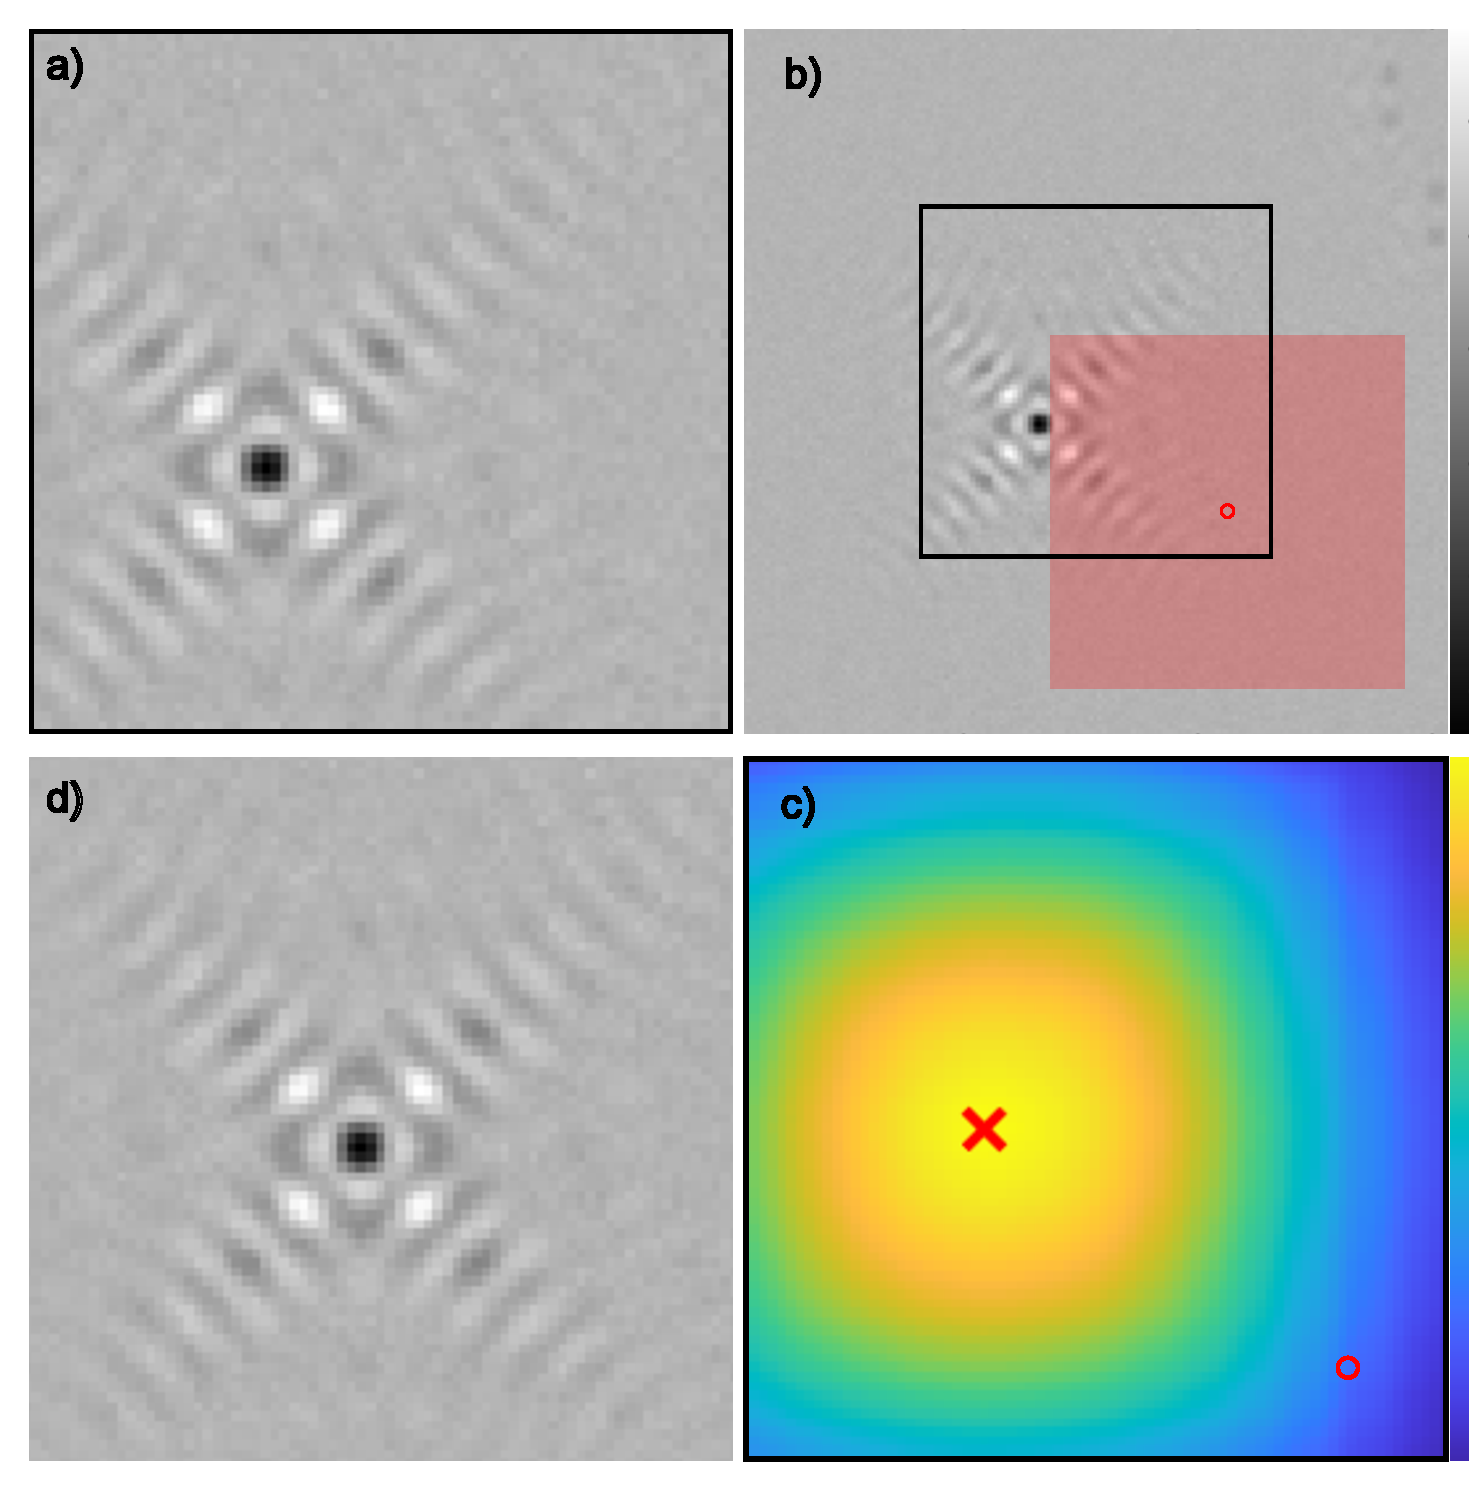
\includegraphics[width= \textwidth]{phase2old.pdf}
	\centering
	\caption{}
	\label{fig:ch6_phase2}
\end{figure}


\begin{figure}
	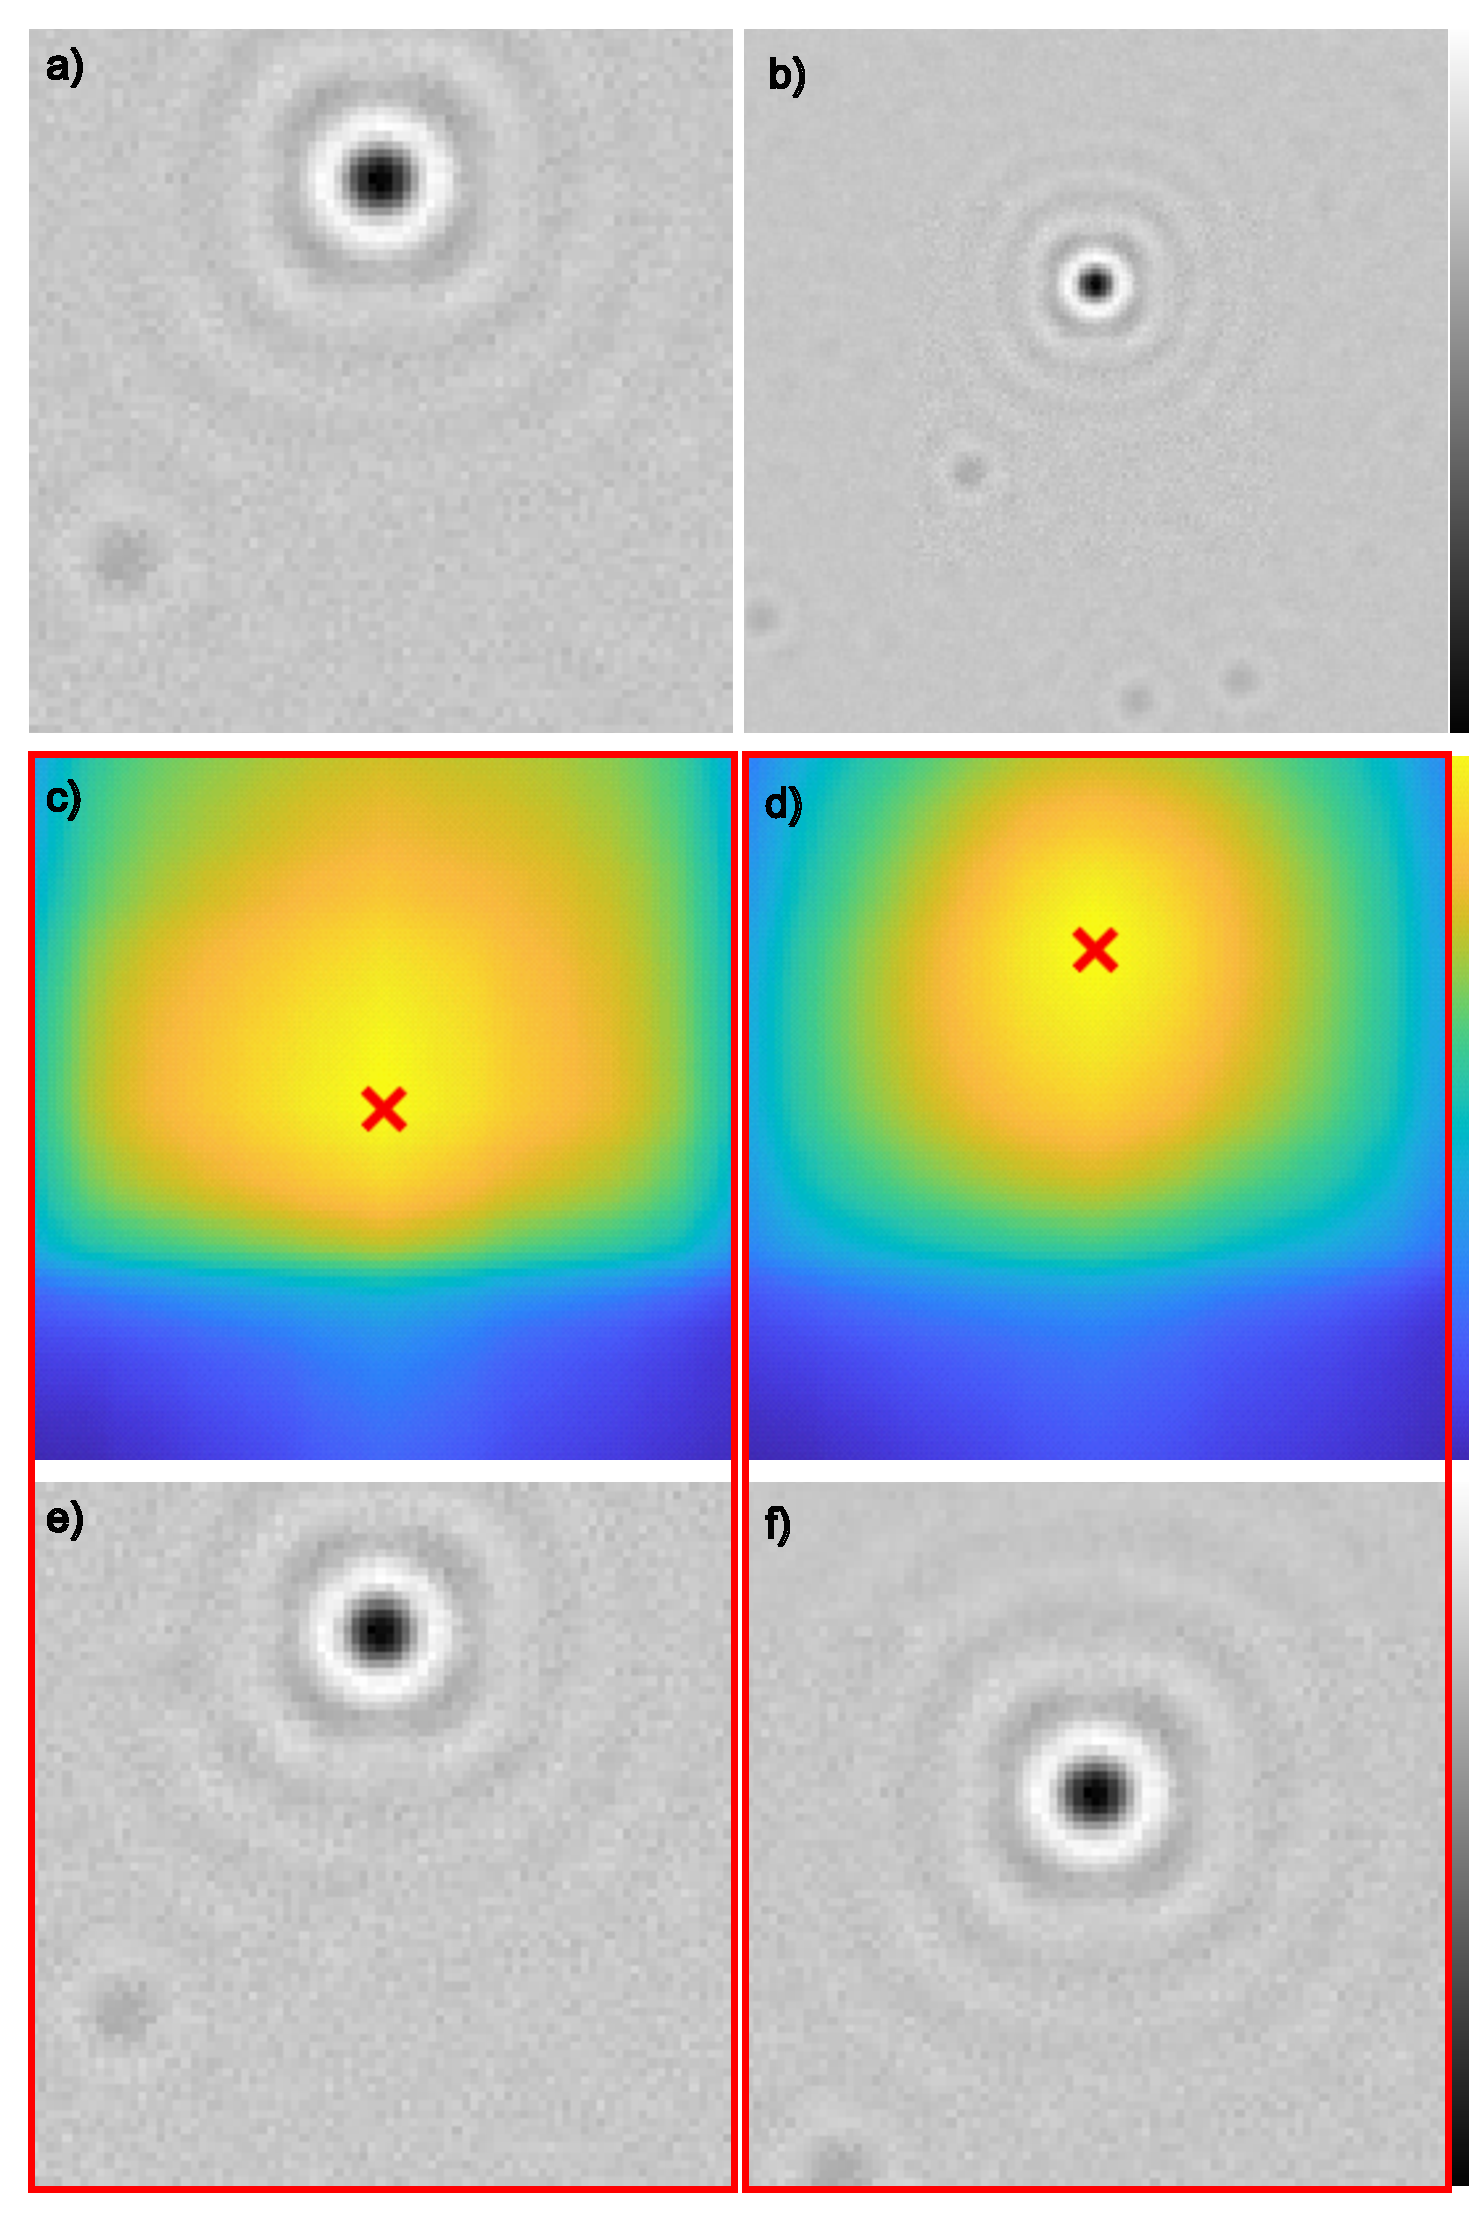
\includegraphics[width= \textwidth]{shifttruncate_mod.pdf}
	\centering
	\caption{}
	\label{fig:ch6_phase2mod}
\end{figure}


\subsection{MC-SBD algorithm}
however, without analytical recovery guarantee, we need metrics and benchmark tests to verify the performance of the algorithm, this part we will elaborate in the next chapter. 
